\chapter{Mobile App (Climber)}
\label{ch:mobile-app}

The Mountain Climber Health \& GPS Tracker mobile application is the primary interface for climbers to interact with their gear. Built with Flutter, it provides real-time health metrics, text messaging capabilities, and location tracking by connecting to the Climber Main Device via Bluetooth Low Energy (BLE).

\section{Installation and Setup}

\subsection{Downloading the Application}
To get started, you must download the latest version of the mobile application from the Summit Gear Portal.

\begin{enumerate}
    \item Log in to your account on the Summit Gear Portal (\url{https://portal.summitgear.com}).
    \item Navigate to the \textbf{Downloads} section.
    \item Download the APK file for Android or follow the TestFlight instructions for iOS.
    \item Install the application on your mobile device.
\end{enumerate}

\subsection{Permissions Configuration}
For the app to function correctly and communicate with the Climber Main Device, you must grant the necessary permissions upon first launch.

\begin{warningbox}
Failure to grant Location and Bluetooth permissions will result in the application being unable to scan for or connect to the Climber Main Device.
\end{warningbox}

\begin{itemize}
    \item \textbf{Bluetooth:} Required for communicating with the ESP32 module on the Climber Main Device.
    \item \textbf{Location:} Required by the operating system for BLE scanning to function correctly.
\end{itemize}

\section{Connecting to the Device}

\subsection{Scanning via BLE}
Ensure that your Climber Main Device is powered on. Open the mobile app and navigate to the \textbf{Devices} tab. 

\begin{enumerate}
    \item Tap the \textbf{Scan for Devices} button.
    \item The app will display a list of available BLE devices nearby.
    \item Look for a device named \texttt{SummitGear\_Climber\_[ID]}.
\end{enumerate}

\subsection{Pairing Process}
Once you locate your device in the list:
\begin{enumerate}
    \item Tap on the device name to initiate pairing.
    \item Upon successful connection, the device status will change to \textbf{Connected}, and the LED indicator on the Climber Main Device will turn solid blue.
\end{enumerate}

\begin{tipbox}
To conserve battery on your mobile device, the app maintains a low-energy connection. However, ensure your phone remains within 10 meters of the Climber Main Device for a stable connection.
\end{tipbox}

\begin{figure}[H]
    \centering
    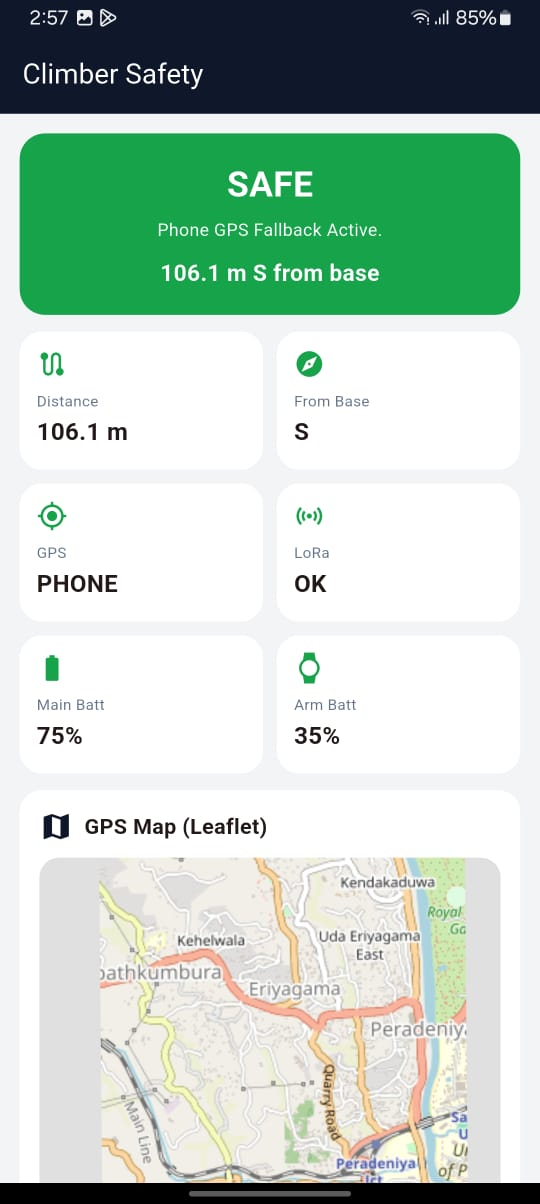
\includegraphics[width=0.8\textwidth]{figures/app-pairing.png}
    \caption{Mobile App Device Scanning and Pairing Screen}
    \label{fig:app-pairing}
\end{figure}

\section{Using the Application}

\subsection{Main Screen Layout}
The main dashboard is designed for high visibility in harsh conditions. It displays critical information at a glance:
\begin{itemize}
    \item \textbf{Health Vitals Panel:} Shows current heart rate, SpO2 levels, and body temperature.
    \item \textbf{Quick Actions:} Buttons for messaging, map view, and settings.
    \item \textbf{Connection Status:} Indicates BLE connection strength and Climber Main Device battery level.
\end{itemize}

\subsection{Viewing Real-Time Vitals}
The vitals are streamed directly from the MAX30102 sensor via the Climber Main Device or the Wristband. 
\begin{itemize}
    \item \textbf{Heart Rate:} Displayed in beats per minute (BPM).
    \item \textbf{SpO2:} Oxygen saturation percentage.
    \item \textbf{Temperature:} Body temperature in Celsius or Fahrenheit (configurable in settings).
\end{itemize}

\begin{infobox}
The health data is updated every 5 seconds to provide near real-time monitoring while optimizing battery life.
\end{infobox}

\subsection{Messaging}
The app allows you to send and receive text messages, which are relayed over the LoRa mesh network via the Climber Main Device.

\begin{enumerate}
    \item Tap the \textbf{Messages} icon on the main screen.
    \item Type your message in the text field (maximum 160 characters).
    \item Tap \textbf{Send}. The message is sent via BLE to the Climber Main Device, which then transmits it over LoRa to the Base Camp or other climbers.
\end{enumerate}

\begin{figure}[H]
    \centering
    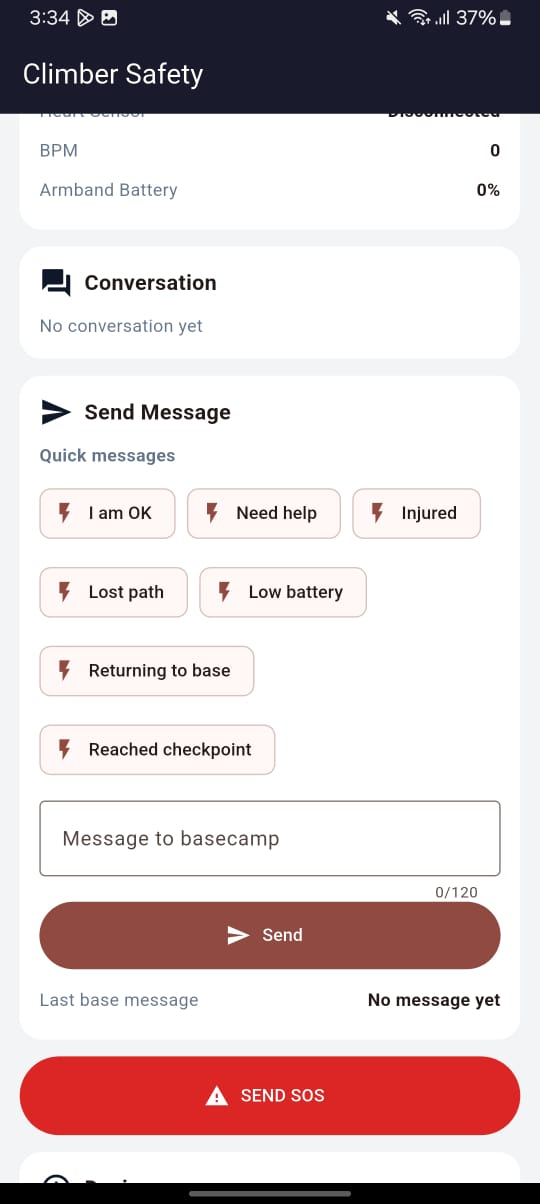
\includegraphics[width=0.8\textwidth]{figures/app-messaging.png}
    \caption{Mobile App Messaging Interface}
    \label{fig:app-messaging}
\end{figure}

\subsection{GPS Location View}
The \textbf{Map} tab utilizes a custom painter to visualize your current GPS coordinates as reported by the NEO-6M module on the Climber Main Device, along with the distance to Base Camp or known waypoints.

\section{OTA Firmware Updates}

The application supports Over-The-Air (OTA) firmware updates to keep your Climber Main Device up to date with the latest features and bug fixes.

\begin{enumerate}
    \item Ensure your Climber Main Device has at least 50\% battery remaining.
    \item In the app, go to \textbf{Settings > Device Maintenance > Firmware Update}.
    \item The app will check the Summit Gear Portal for available updates (requires internet connection).
    \item If an update is available, tap \textbf{Download \& Install}.
    \item The app will transfer the firmware via BLE. \textbf{Do not close the app or disconnect the device during this process.}
\end{enumerate}

\begin{cautionbox}
Interrupting an OTA update may corrupt the firmware on the Climber Main Device. Ensure a stable connection and sufficient battery before proceeding.
\end{cautionbox}
